\section{Results}
\label{sec:psunc:results}
The events generated by the tools of Sec.~\ref{sec:psunc:tools} were analysed
with \textsc{Rivet} \cite{Buckley:2010ar} using three custom analyses. The
analysis for $e^+e^-$, is closely derived from \textsc{ALEPH\_2004\_S5765862}
\cite{Heister:2003aj} which contains descriptions of the observables
studied. The $pp$ results were produced using analyses that closely follow
content of \textsc{MC\_HINC}/\textsc{MC\_HJETS}. The jets definitions used in
all of these analyses are implemented in \textsc{FastJet}
\cite{Cacciari:2011ma}.

We investigate three separate processes at leading order with two different
scenarios. In sections \ref{sec:psunc:results:ee}-\ref{sec:psunc:results:z} we
display a selection of plots for discussion. The content of the uncertainty
bands for each generator are described in Sec.~\ref{sec:psunc:tools}

\subsection{$e^+e^-\to\text{jets}$}
\label{sec:psunc:results:ee}
This process is a natural starting point to explore shower uncertainties as we
only encounter final state radiation. For this process, the two scenarios
correspond to CoM energies of $\sqrt{s}=91\GeV$ and $\sqrt{s}=500\GeV$. The
jets are defined by the Durham jet algorithm with $y_\mathrm{cut}=0.7$. From
the analysis we present a subset of the event shape observables and jet
fractions. The results of both scenarios yielded similar conclusions and
we will omit the $500\GeV$ results with one exception.
\begin{figure}[h]
  \centering
  \begin{subfigure}[t]{0.49\textwidth}
    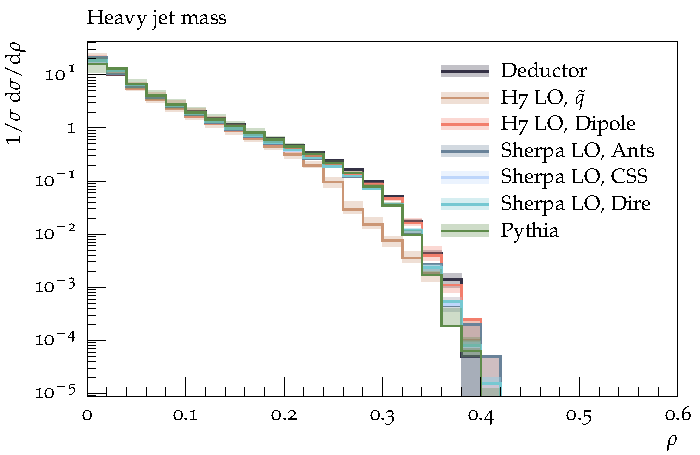
\includegraphics[width=\textwidth]{plots/EE-91-MuShower/MC_EETOJETS/HeavyJetMass.pdf}
    \caption{$\sqrt{s} = 91\GeV$}
    \label{fig:ee:heavyjetmass:91}
  \end{subfigure}
  %
  \begin{subfigure}[t]{0.49\textwidth}
    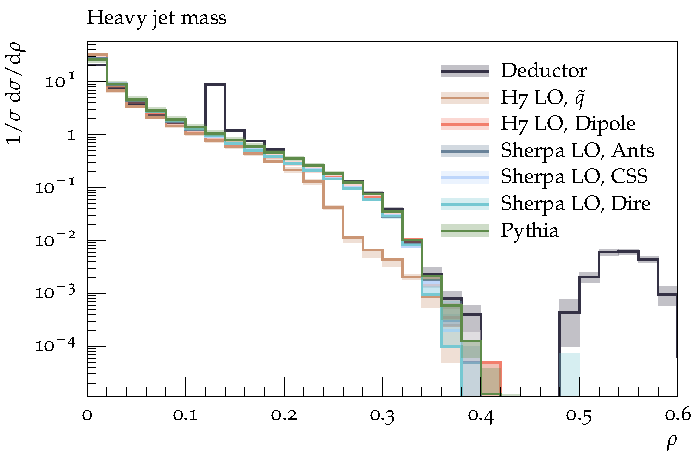
\includegraphics[width=\textwidth]{plots/EE-500-MuShower/MC_EETOJETS/HeavyJetMass.pdf}
    \caption{$\sqrt{s} = 500\GeV$}
    \label{fig:ee:heavyjetmass:500}
  \end{subfigure}
  \caption{Comparison of Heavy Jet mass at two different energies.}
  \label{fig:ee:heavyjetmass}
\end{figure}

The predictions for the heavy jet mass, Fig.~\ref{fig:ee:heavyjetmass}, show
consistency over the majority of the distribution as well as consistent
predictions for the size of the uncertainty bands.  The \Deductor curve for
$\rho$ at $500\GeV$ has two features of interest; these stem from the
$t\bar{t}$ contribution without the top decay. The new features emerge from
the heavy jet containing 1 or 2 of the un-decayed top quarks.

\begin{figure}[h]
  \centering
  \begin{minipage}[t]{0.4c9\textwidth}
    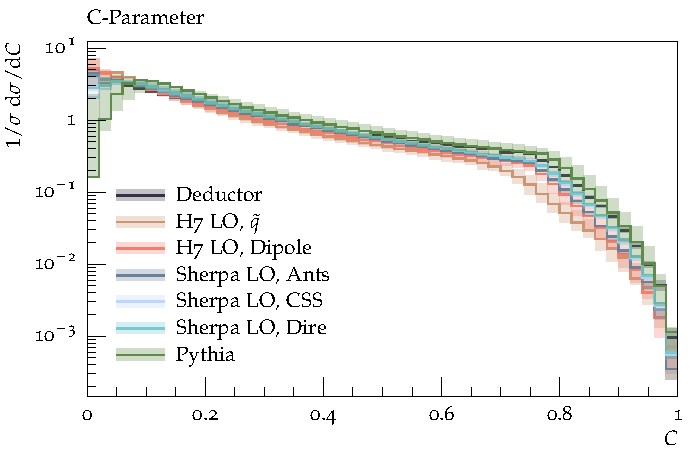
\includegraphics[width=1\textwidth]{plots/EE-91-MuShower/MC_EETOJETS/CParameter.pdf}
    \caption{C-parameter at $\sqrt{s}=91\GeV$.}
    \label{fig:ee:cparam:91}
  \end{minipage}
  %
  \begin{minipage}[t]{0.49\textwidth}
    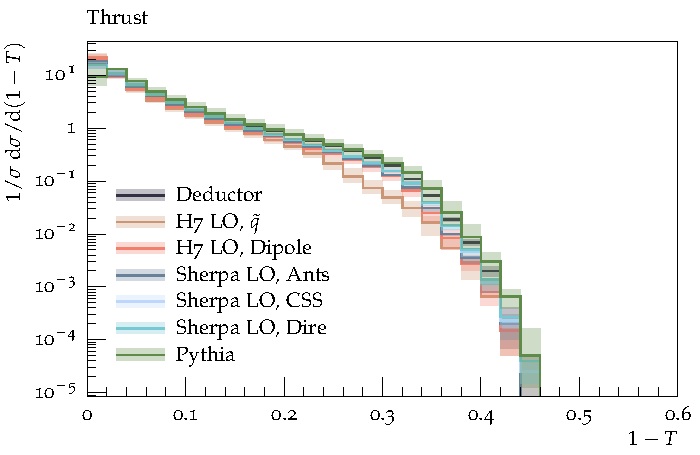
\includegraphics[width=1\textwidth]{plots/EE-91-MuShower/MC_EETOJETS/Thrust.pdf}
    \caption{Thrust at $\sqrt{s}=91\GeV$.}
	\label{fig:ee:thrust:91}
  \end{minipage}
\end{figure}

The \Herwig \QTilde ``dead-zone'' can be seen in 
Fig.~\ref{fig:ee:heavyjetmass}-\ref{fig:ee:thrust:91} and
Fig.~\ref{fig:ee:r1:91}.  The C-parameter, Fig.~\ref{fig:ee:cparam:91}, has
reasonable agreement over the majority of the distribution but differences are
evident in its behaviour near $C=0$, and in the region $C>3/4$. As the region
$C>3/4$ is driven by non-planar events, which contain multiple emissions, it
is sensitive to the shower implementation and differences should be expected.
This same is true for Thrust, Fig.~\ref{fig:ee:thrust:91}, which again shows
good agreement over the majority of the distribution, and differences that do
emerge are in regions that are sensitive to multiple emissions, or as we
approach the dijet configuration.
\begin{figure}[h]
  \centering
  \begin{subfigure}[t]{0.49\textwidth}
    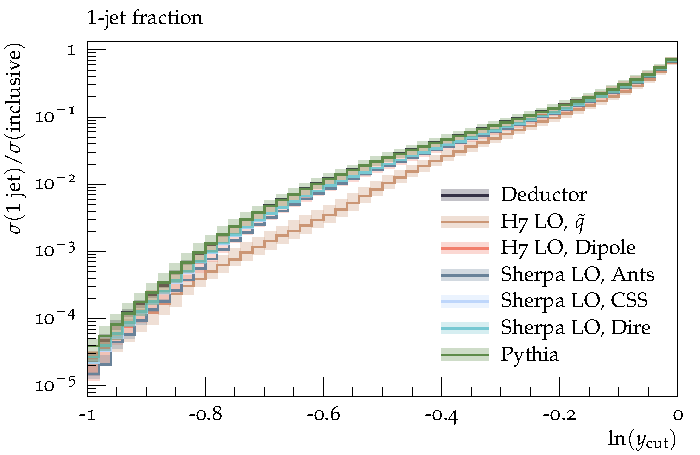
\includegraphics[width=1\textwidth]{plots/EE-91-MuShower/MC_EETOJETS/R1.pdf}
    \caption{1-jet fraction}
    \label{fig:ee:r1:91}
  \end{subfigure}
  %
  \begin{subfigure}[t]{0.49\textwidth}
    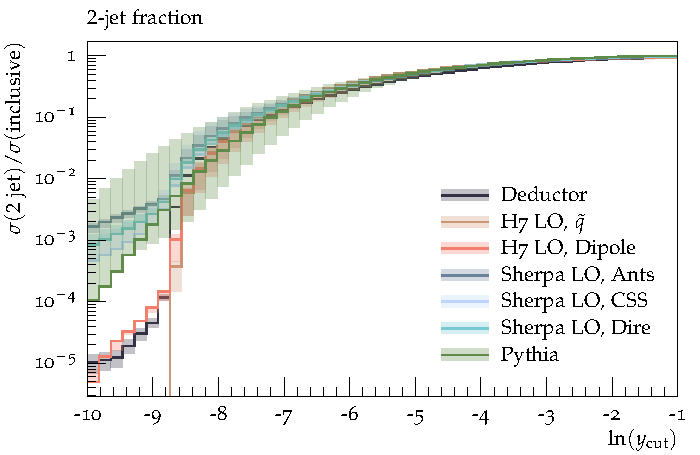
\includegraphics[width=1\textwidth]{plots/EE-91-MuShower/MC_EETOJETS/R2.pdf}
    \caption{2-jet fraction}
    \label{fig:ee:r2:91}
  \end{subfigure}
  \caption{Jet fractions at $\sqrt{s}=91\GeV$.}
  \label{fig:ee:r:91}
\end{figure}
Aside from \Herwig \QTilde, the results for the 1-jet fraction are in good
agreement within uncertainty bands. For the 2-jet fraction we see the
differences that come from the implementation of the shower cutoff. There is
also a large disagreement on the size of the uncertainty bands reported; here
the choice of evolution variable can cause the shower to probe much smaller
values of $p_\perp$. In this region we should expect some interplay with
hadronization and, though beyond the aim of this study, this merits further
investigation.

\subsection{$pp\to h$}
\label{sec:psunc:results:h}
Higgs production (via HEFT) presents two new aspects: initial-state radiation,
and the gluon PDF. The simulations take place at $\sqrt{s}=13~\mathrm{TeV}$,
and the analysis considers anti-$k_T$ jets with $p_\perp\geq 40\GeV$. We
explore two scenarios $m_H=125\GeV$ and $m_H=500\GeV$ to quantify the impact of
the hard scalex. However, we neglect to show the heavy Higgs results, as they
offer no new insight.

\begin{figure}[h]
  \centering
  \begin{subfigure}[t]{0.49\textwidth}
    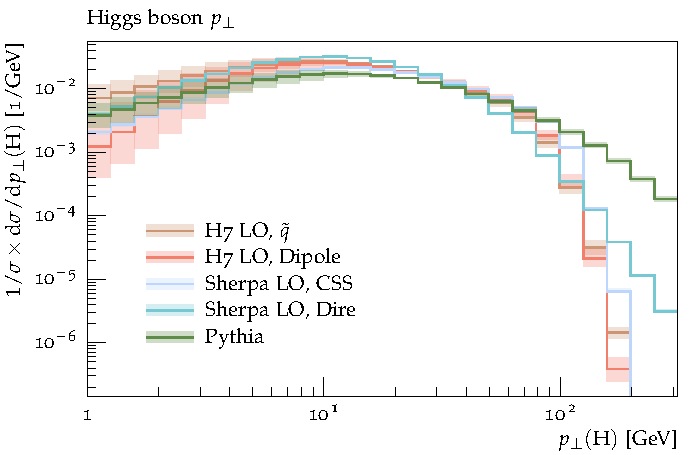
\includegraphics[width=\textwidth]{plots/H-125-MuShower/LH_H/X_pT.pdf}
    \caption{Entire Region}
    \label{fig:h:pt_full}
  \end{subfigure}
%
  \begin{subfigure}[t]{0.49\textwidth}
    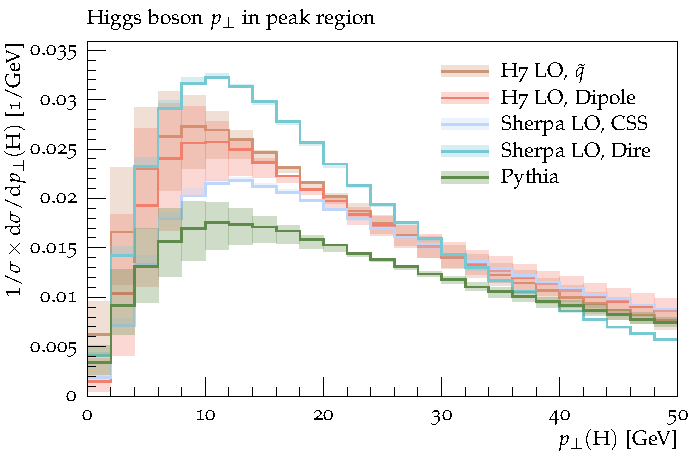
\includegraphics[width=\textwidth]{plots/H-125-MuShower/LH_H/X_pT_peak.pdf}
    \caption{Peak Region}
    \label{fig:h:pt_peak}
  \end{subfigure}
  \caption{Generator comparison of the $H$ $p_\perp$ showing the overall
    behaviour \ref{fig:h:pt_full} as well as the behaviour in the peak region
    \ref{fig:h:pt_peak}}
  \label{fig:h:pt}
\end{figure}

\begin{figure}[h]
  \centering
  \begin{minipage}[t]{0.49\textwidth}
    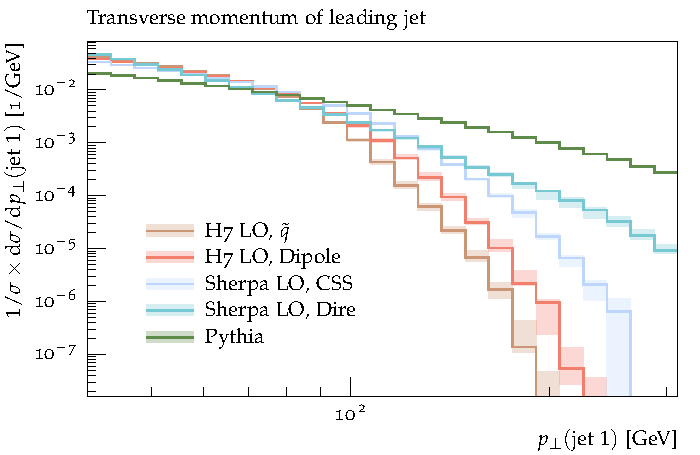
\includegraphics[width=1\textwidth]{plots/H-125-MuShower/LH_H/jet1_pT.pdf}
    \caption{$p_\perp$ of the leading jet}
    \label{fig:h:jet1_pt}
  \end{minipage}
  %
  \begin{minipage}[t]{0.49\textwidth}
    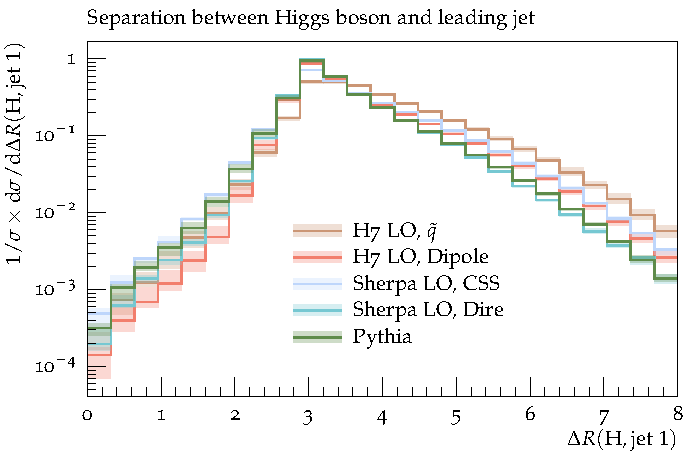
\includegraphics[width=1\textwidth]{plots/H-125-MuShower/LH_H/X_jet1_dR.pdf}
    \caption{Comparison for the lego-plot distance between the Higgs and the leading jet}
    \label{fig:h:deltaR}
  \end{minipage}
\end{figure}

\begin{figure}[h]
  \centering
  \begin{minipage}[t]{0.49\textwidth}
    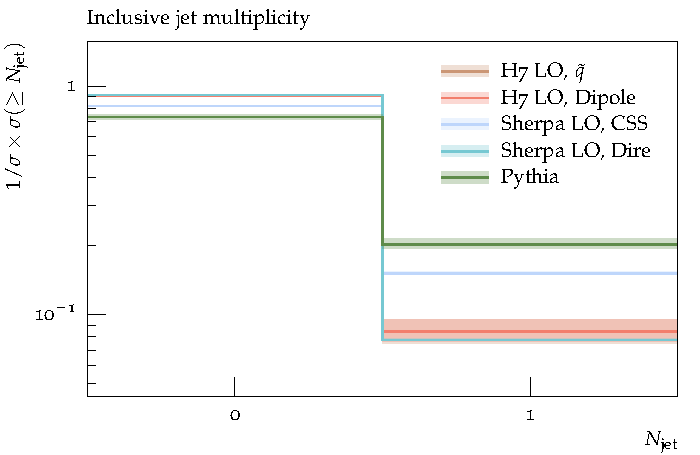
\includegraphics[width=1\textwidth]{plots/H-125-MuShower/LH_H/jet_multi_inclusive.pdf}
    \caption{Comparison for inclusive jet multiplicity}
    \label{fig:h:jet_multi_inc}
  \end{minipage}
  %
  \begin{minipage}[t]{0.49\textwidth}
    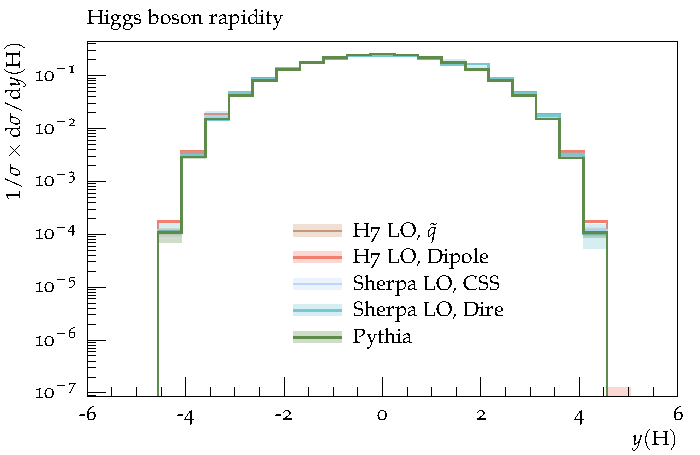
\includegraphics[width=1\textwidth]{plots/H-125-MuShower/LH_H/X_y.pdf}
    \caption{Higgs rapidity}
    \label{fig:h:y}
  \end{minipage}
\end{figure}

The $p_\perp$ distributions for the Higgs, Fig.~\ref{fig:h:pt}, have good
agreement at low $p_\perp$ and expectedly disagree at high $p_\perp$, where
the differences are not reflected in the uncertainty bands. In the peak region
further differences are also apparent, and can be attributed to different
shower implementations: evolution variable, $\alpha_s$ and intrinsic $k_T$,
and recoil. The high $p_\perp$ behaviour of \Herwig and \Sherpa \CSS are
closer to the scale $m_H$, while \Pythia and \Sherpa \Dire extend further and
probe the phase space of a power-shower setup. The agreement displayed between
the different \Herwig showers is expected from the setup, nevertheless it is a
satisfying result given their different implementations.  The leading jet
$p_\perp$, Fig.~\ref{fig:h:jet1_pt}, is consistent at low $p_\perp$ with the
exception of \Pythia, which has a notably harder distribution. Though the high
$p_\perp$ predictions are markedly different, \Herwig and \Sherpa \CSS do
again show the same suppression near the scale $m_H$; the harder jets produced
by a power-shower can clearly be seen here.  The lego-distance,
Fig.~\ref{fig:h:deltaR}, has two notable regions $\Delta R \geq\pi$ and
$\Delta R < \pi$. For the first region, we see that the generators give
differing predictions with small uncertainty bands, this region is typically
driven by few hard-emissions. The second region, driven by multiple emissions,
displays better agreement and, expectedly, has larger uncertainty bands.  The
inclusive jet multiplicity shows some agreement between generators, but
notably \Sherpa \CSS and \Pythia produce a smaller fraction of $0$-jet
events. Finally, we show the resilience of an inclusive observable to the
shower, and its uncertainties. This can be seen in the Higgs rapidity,
Fig.~\ref{fig:h:y}.

\subsection{$pp\to Z$}
\label{sec:psunc:results:z}
To complement the previous process a quark-initiated setup is presented, again
using two different hard scales of $91\ {\rm GeV}$ and $500\ {\rm GeV}$. The
analysis and findings of this section are similar to that of
Sec.~\ref{sec:psunc:results:h}. The predictions for the inclusive jet
multiplicity, Fig.~\ref{fig:z:jet_multi_inc}, are much less consistent
Fig.~\ref{fig:h:jet_multi_inc}.
\begin{figure}[h]
  \centering
    \begin{subfigure}[t]{0.49\textwidth}
    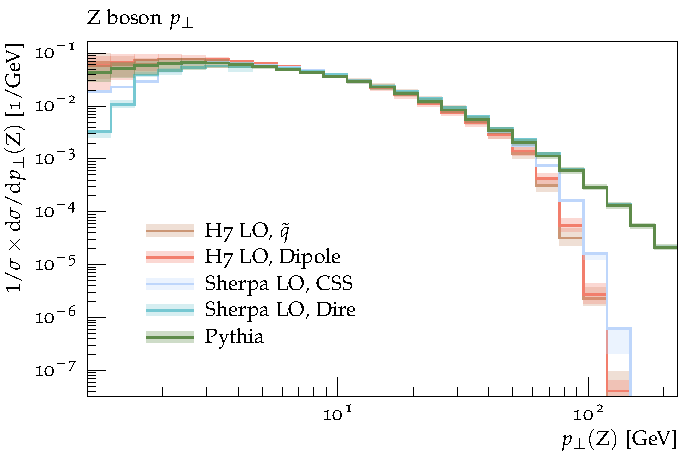
\includegraphics[width=\textwidth]{plots/Z-91-MuShower/LH_Z/X_pT.pdf}
    \caption{Entire region}
    \label{fig:z:pt_full}
  \end{subfigure}
%
  \begin{subfigure}[t]{0.49\textwidth}
    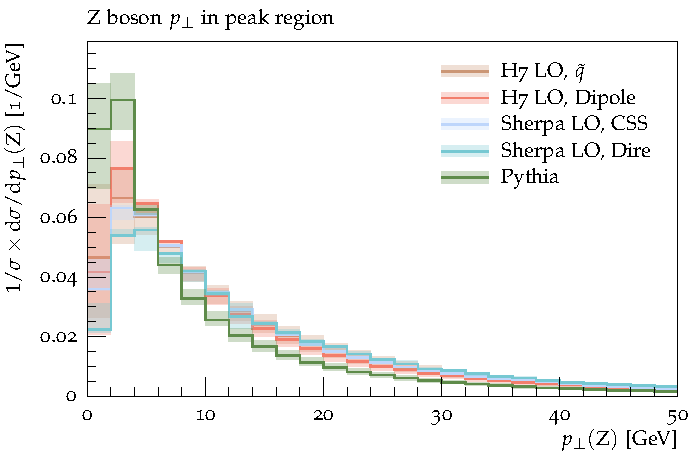
\includegraphics[width=\textwidth]{plots/Z-91-MuShower/LH_Z/X_pT_peak.pdf}
    \caption{Peak region}
    \label{fig:z:pt_peak}
  \end{subfigure}
  \caption{Generator comparison of the $Z$ $p_\perp$ showing the overall behaviour \ref{fig:z:pt_full} as well as the behaviour in the peak region \ref{fig:z:pt_peak}.}
  \label{fig:z:pt}
\end{figure}

\begin{figure}[h]
  \centering
  \begin{minipage}[t]{0.49\textwidth}
    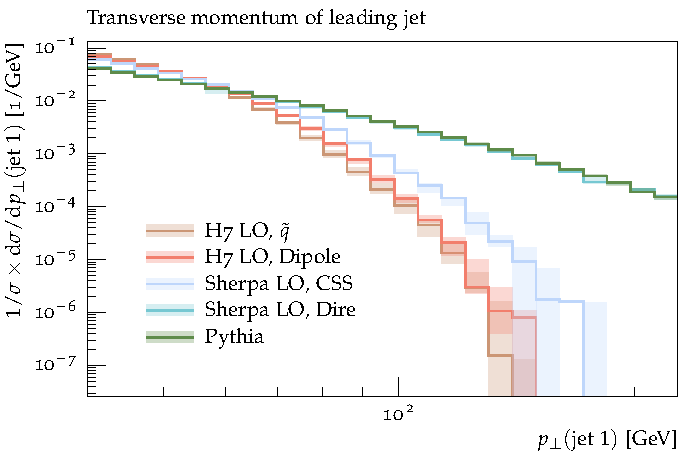
\includegraphics[width=1\textwidth]{plots/Z-91-MuShower/LH_Z/jet1_pT.pdf}
    \caption{$p_\perp$ of the leading jet}
    \label{fig:z:jet1_pt}
  \end{minipage}
  %
  \begin{minipage}[t]{0.49\textwidth}
    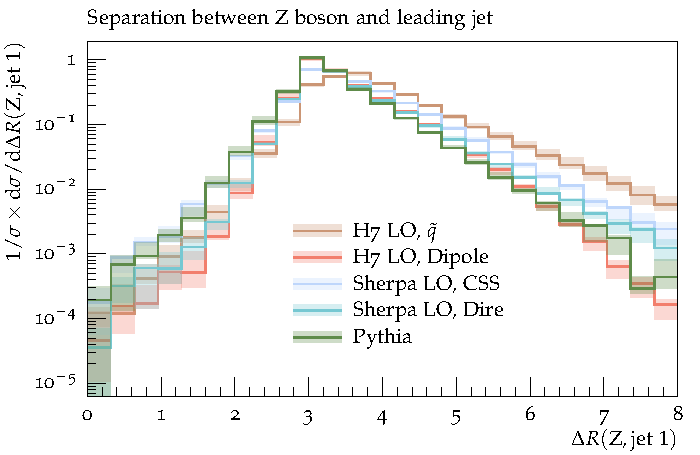
\includegraphics[width=1\textwidth]{plots/Z-91-MuShower/LH_Z/X_jet1_dR.pdf}
    \caption{Lego-plot distance between the $Z$ and the leading jet}
    \label{fig:z:deltaR}
  \end{minipage}
\end{figure}

\begin{figure}[h]
  \centering
  \begin{minipage}[t]{0.49\textwidth}
    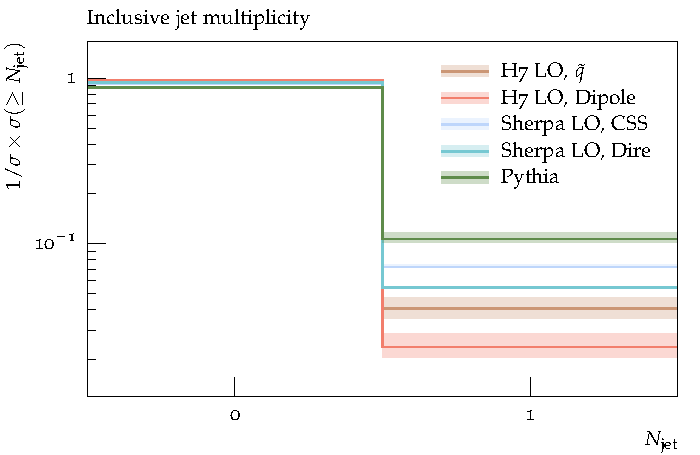
\includegraphics[width=1\textwidth]{plots/Z-91-MuShower/LH_Z/jet_multi_inclusive.pdf}
    \caption{Inclusive jet multiplicity}
    \label{fig:z:jet_multi_inc}
  \end{minipage}
  %
  \begin{minipage}[t]{0.49\textwidth}
    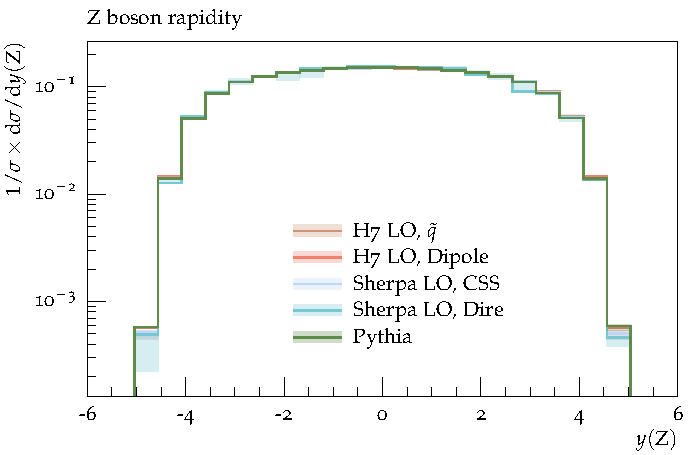
\includegraphics[width=1\textwidth]{plots/Z-91-MuShower/LH_Z/X_y.pdf}
    \caption{$Z$ rapidity}
    \label{fig:z:y}
  \end{minipage}
\end{figure}
